\begin{figure}
\centering
%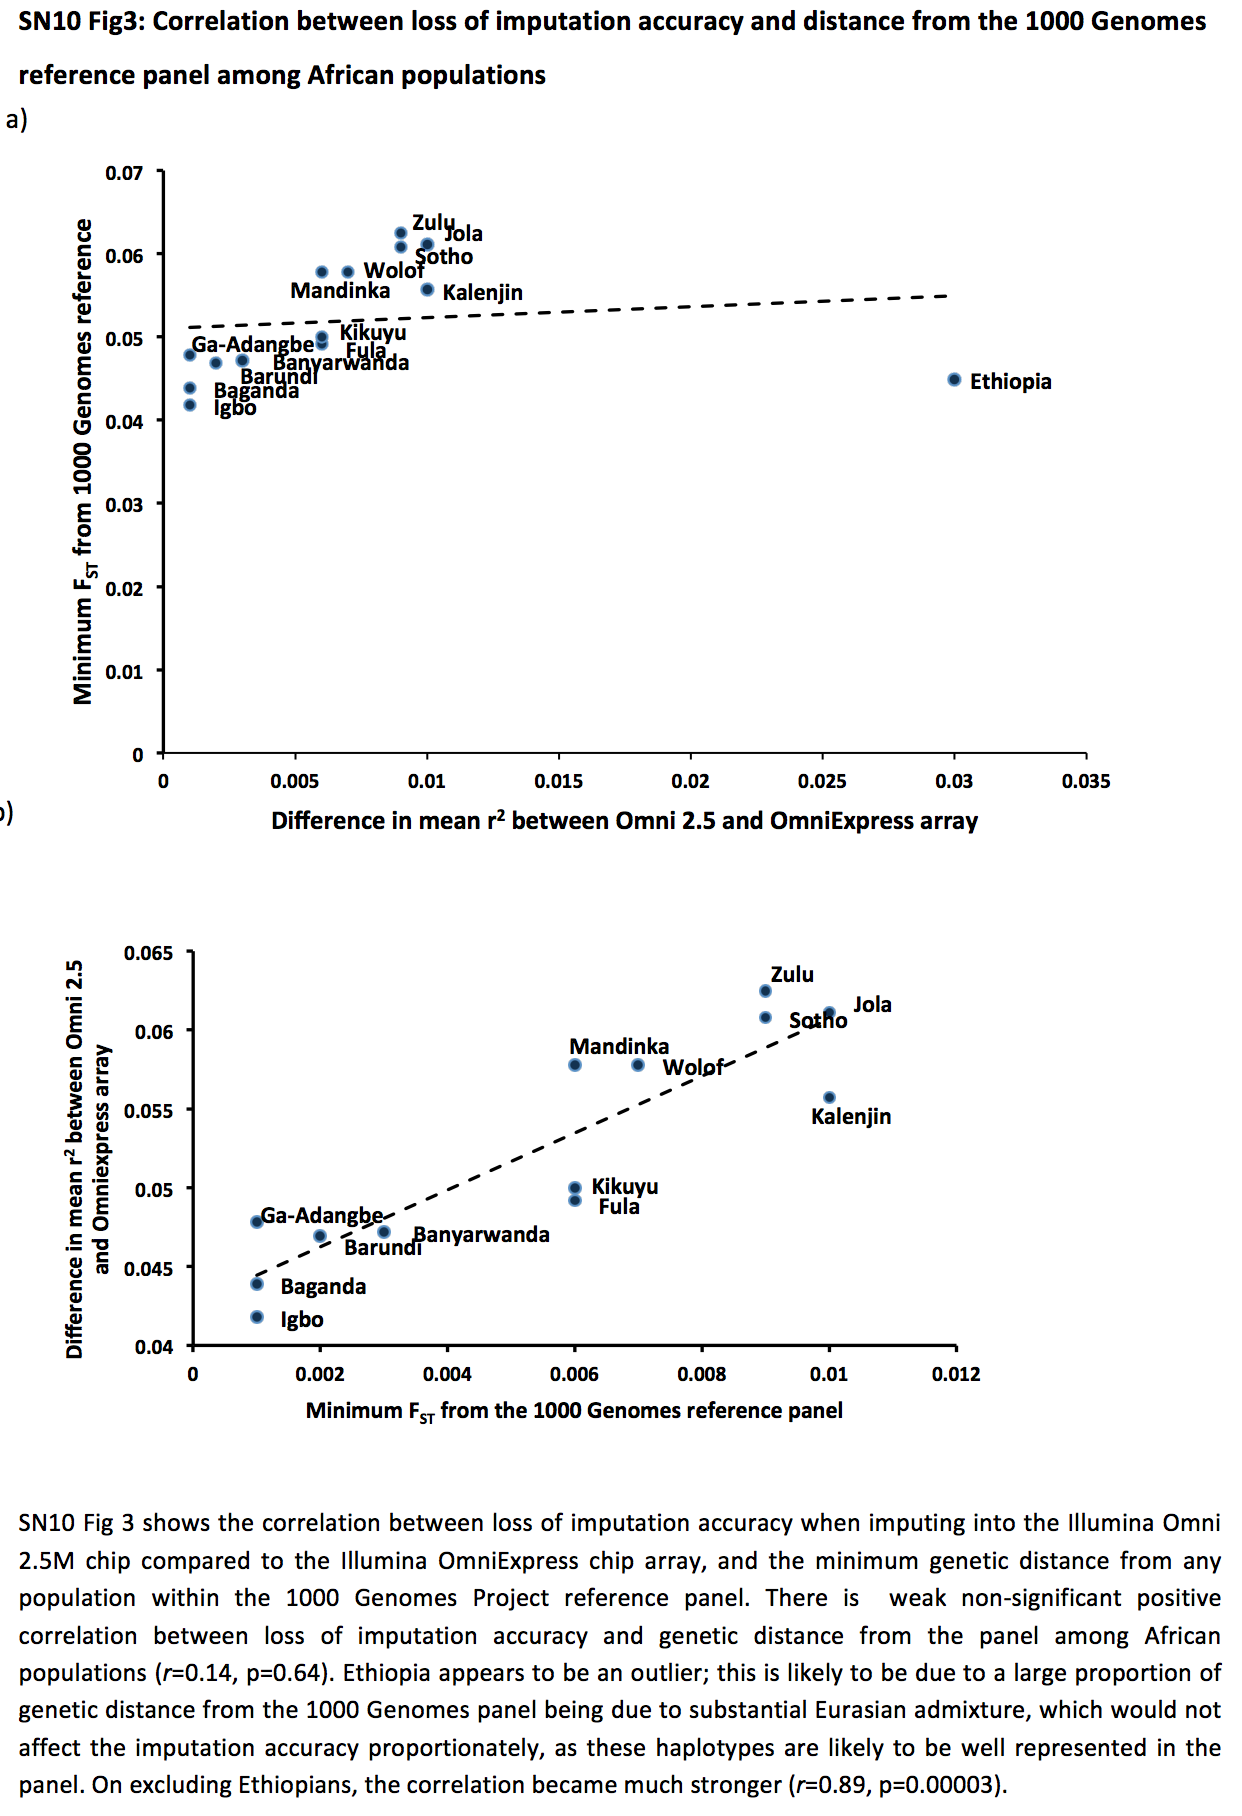
\includegraphics[trim={0.5cm 6.5cm 0cm 2cm},clip,width=0.75\textwidth]{fig/SN10f3}
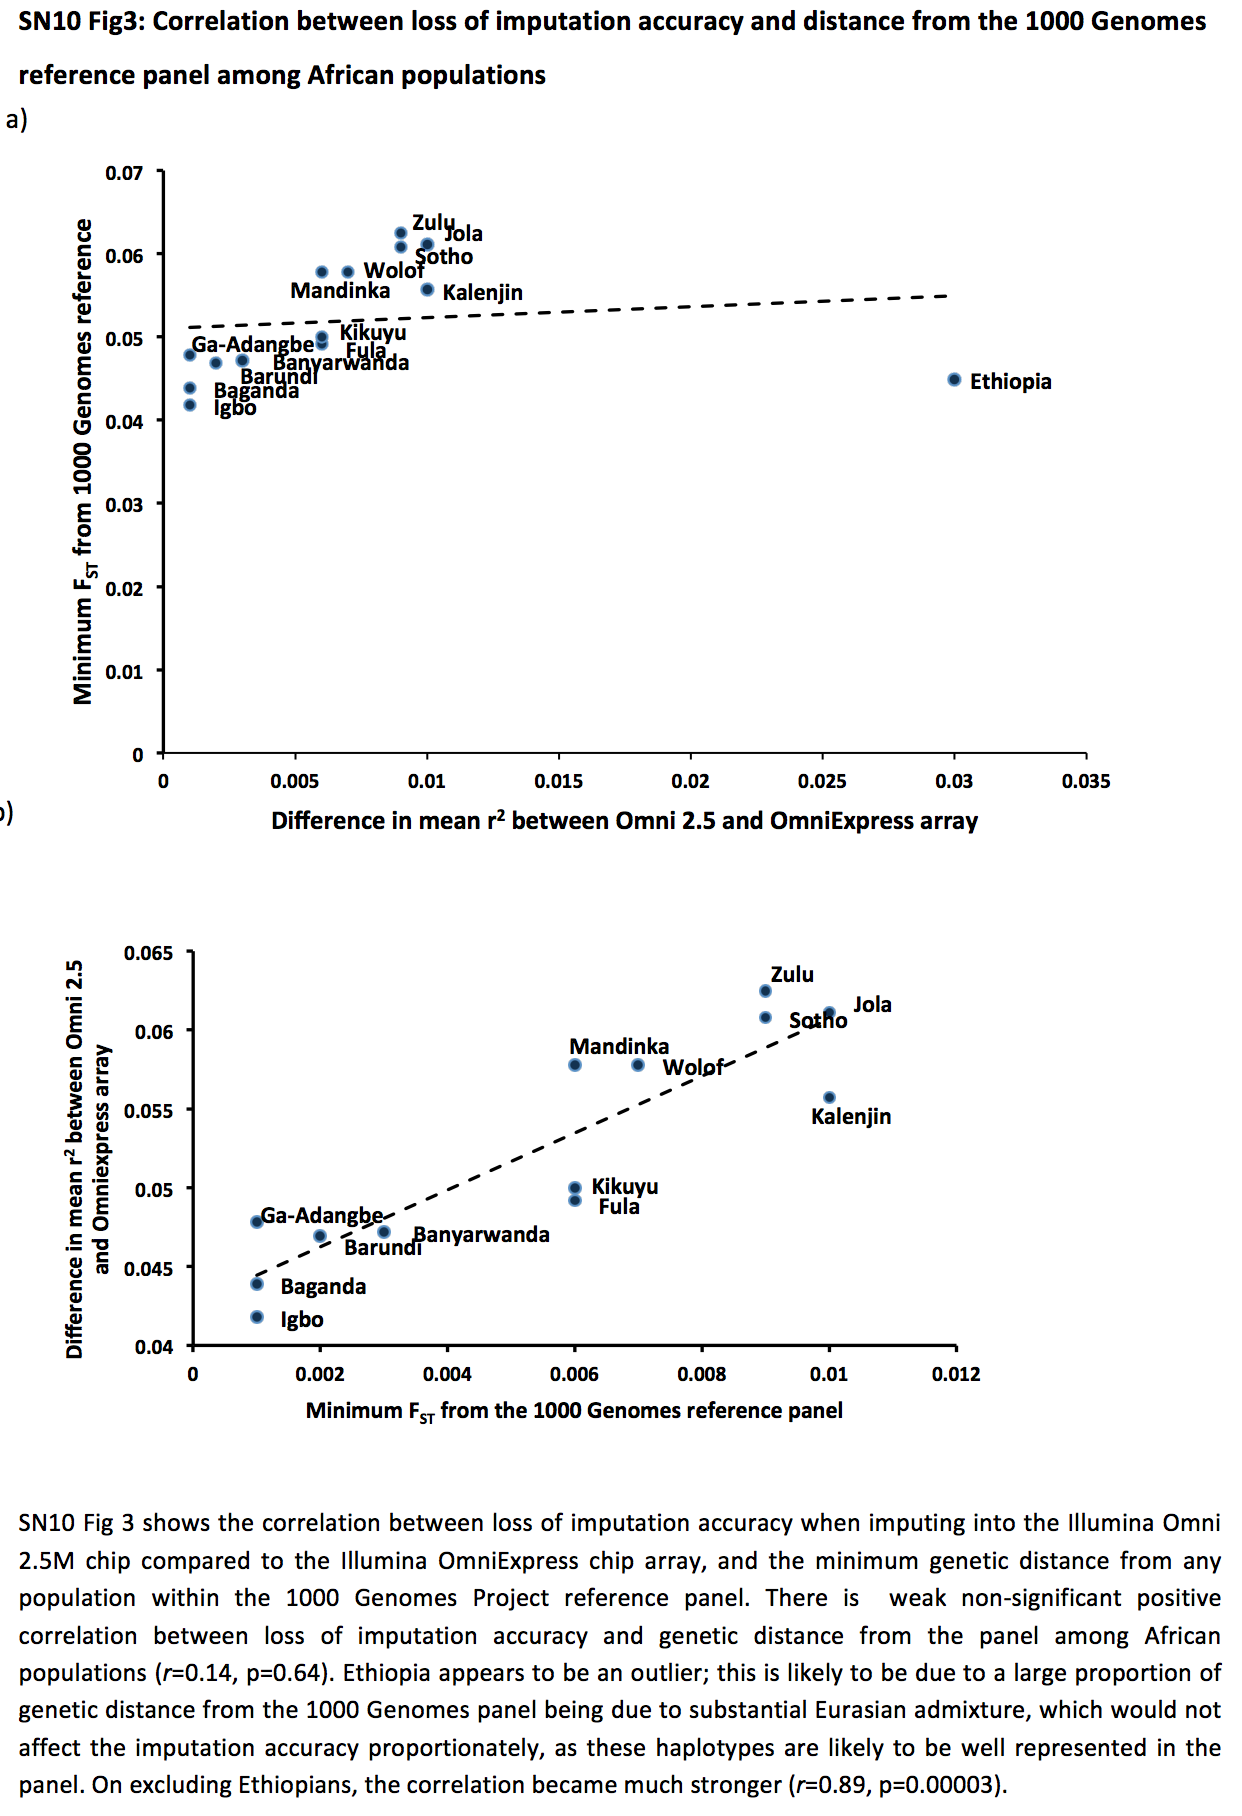
\includegraphics[trim={0.5cm 6.5cm 0cm 15cm},clip,width=0.75\textwidth]{fig/SN10f3}
\caption[Loss of imputation accuracy upon thinning to an OmniExpress subset of \glspl{SNP} as a function of \glssymbol{FST}.]{Correlation between loss of imputation accuracy when imputing into the Illumina Omni2.5M chip compared to the Illumina OmniExpress chip array, and the minimum genetic distance from any population within the \gls{1000G} reference panel. There is weak non-significant positive correlation between loss of imputation accuracy and genetic distance from the panel among African populations (\textit{r}=0.14, \textit{p}=0.64). Ethiopia appears to be an outlier; this is likely to be due to a large proportion of genetic distance from the \gls{1000G} panel being due to substantial Eurasian admixture, which would not affect the imputation accuracy proportionately, as these haplotypes are likely to be well represented in the panel. The Ethiopians have also been pooled from 5 different sub-populat, which makes the accuracy of the \glssymbol{FST} uncertain. On excluding Ethiopians, the correlation became much stronger (\textit{r}=0.89, \textit{p}=0.00003). \glssymbol{FST} values calculated by Deepti Gurdasani and Savita Karthikeyan. Correlation coefficient and probability of correlation calculated by Deepti Gurdasani.}
\label{fig:SN10f3}
\end{figure}